\documentclass[10pt, twocolumn]{article}
\usepackage[utf8]{inputenc}
\usepackage{graphicx}
\usepackage[english]{babel}
\usepackage{hyperref}
\usepackage{fancyhdr}

\hypersetup{
    colorlinks=true,
    linkcolor=blue,
    filecolor=magenta,      
    urlcolor=cyan,
}
\graphicspath{ {images/} }


\title{\vspace{-4cm}Application Architectures}
\author{Kelsey McKenna}
\date{}

\begin{document}
\pagenumbering{gobble}
\maketitle

Credit to \href{https://dzone.com/articles/onion-architecture-is-interesting}{Grzegorz Ziemoński}

\section*{Layered}

\begin{center}
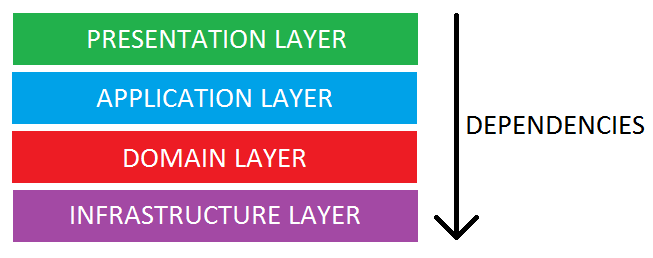
\includegraphics[width=0.45\textwidth]{layered-architecture-overview.png}
\end{center}

\section*{Hexagonal}

\begin{center}
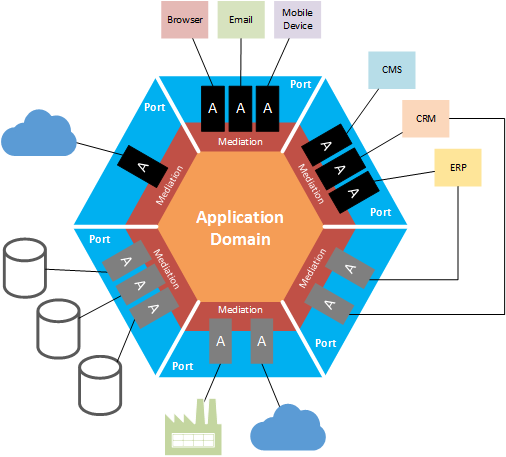
\includegraphics[width=0.45\textwidth]{hexagonal.png}
\end{center}


\begin{itemize}
    \item Ports and adapters -- interfaces and implementations
\end{itemize}

\section*{Onion}

\begin{center}
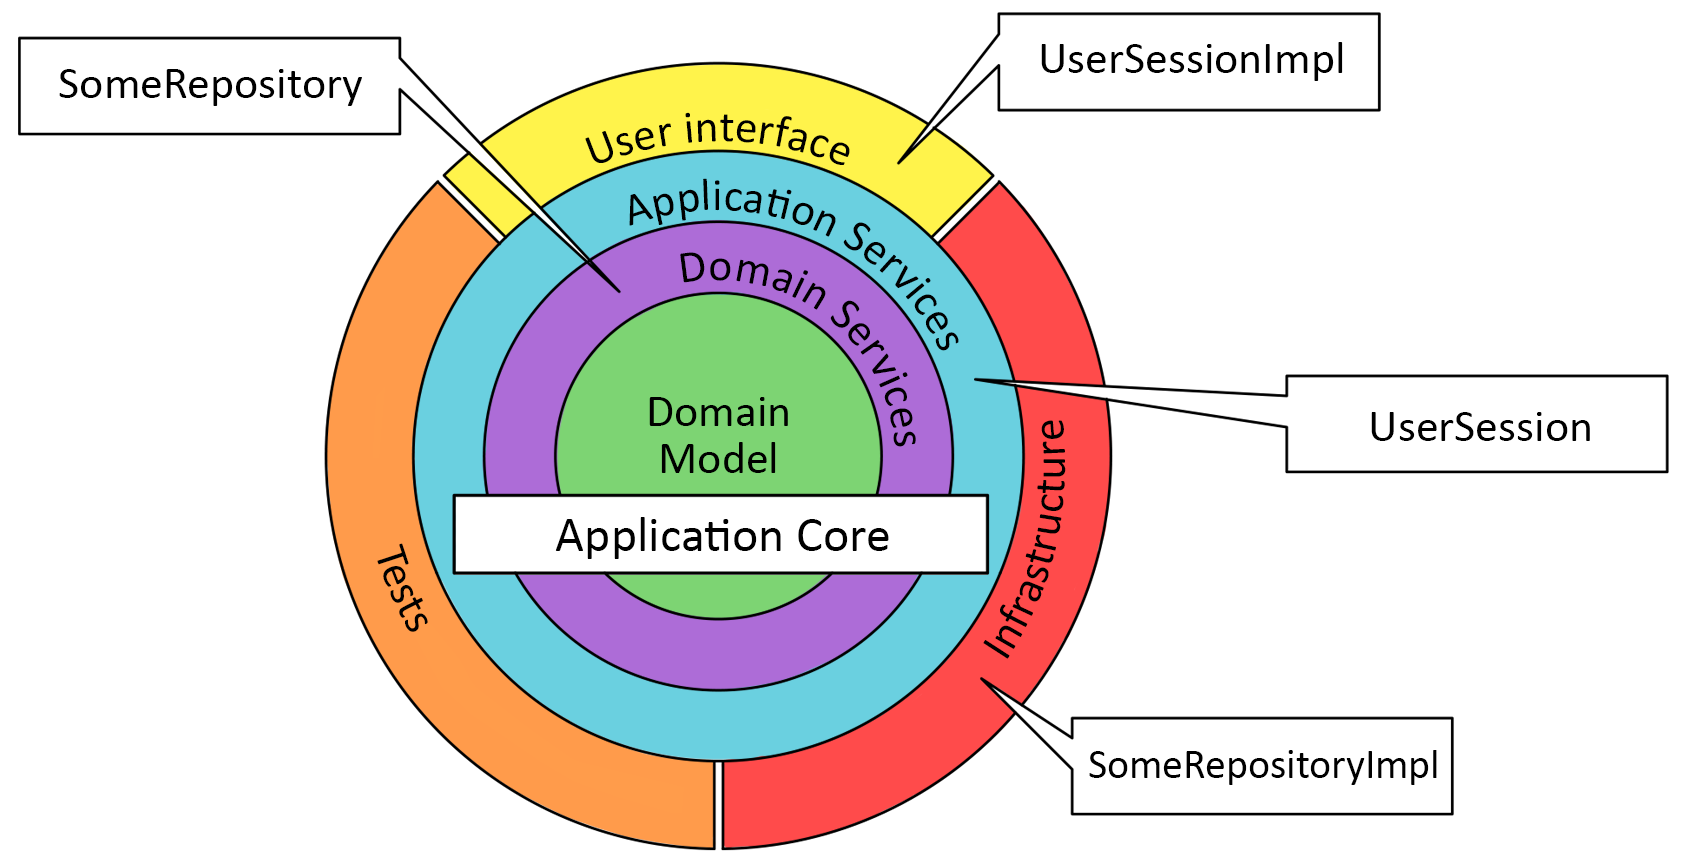
\includegraphics[width=0.45\textwidth]{onion.png}
\end{center}

\begin{itemize}
    \item \textbf{Domain Model layer}, where our entities and classes closely related to them e.g. value objects reside.
    \item \textbf{Domain Services layer}, where domain-defined processes reside.
    \item \textbf{Application Services layer}, where application-specific logic i.e. our use cases reside.
    \item \textbf{Outer layer}, which keeps peripheral concerns like UI, databases or tests.
\end{itemize}

\section*{Package by Feature}

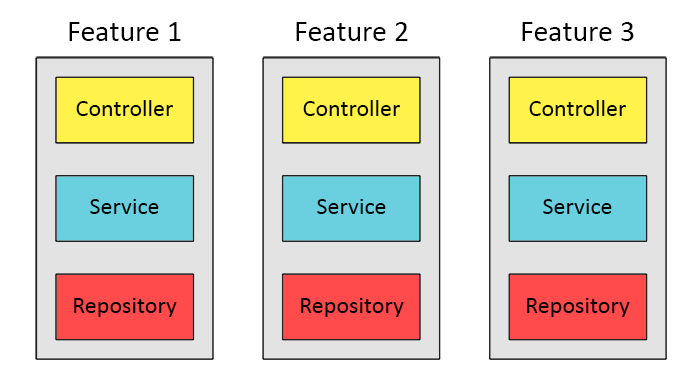
\includegraphics[width=0.45\textwidth]{package-by-feature.png}

\section*{Clean}

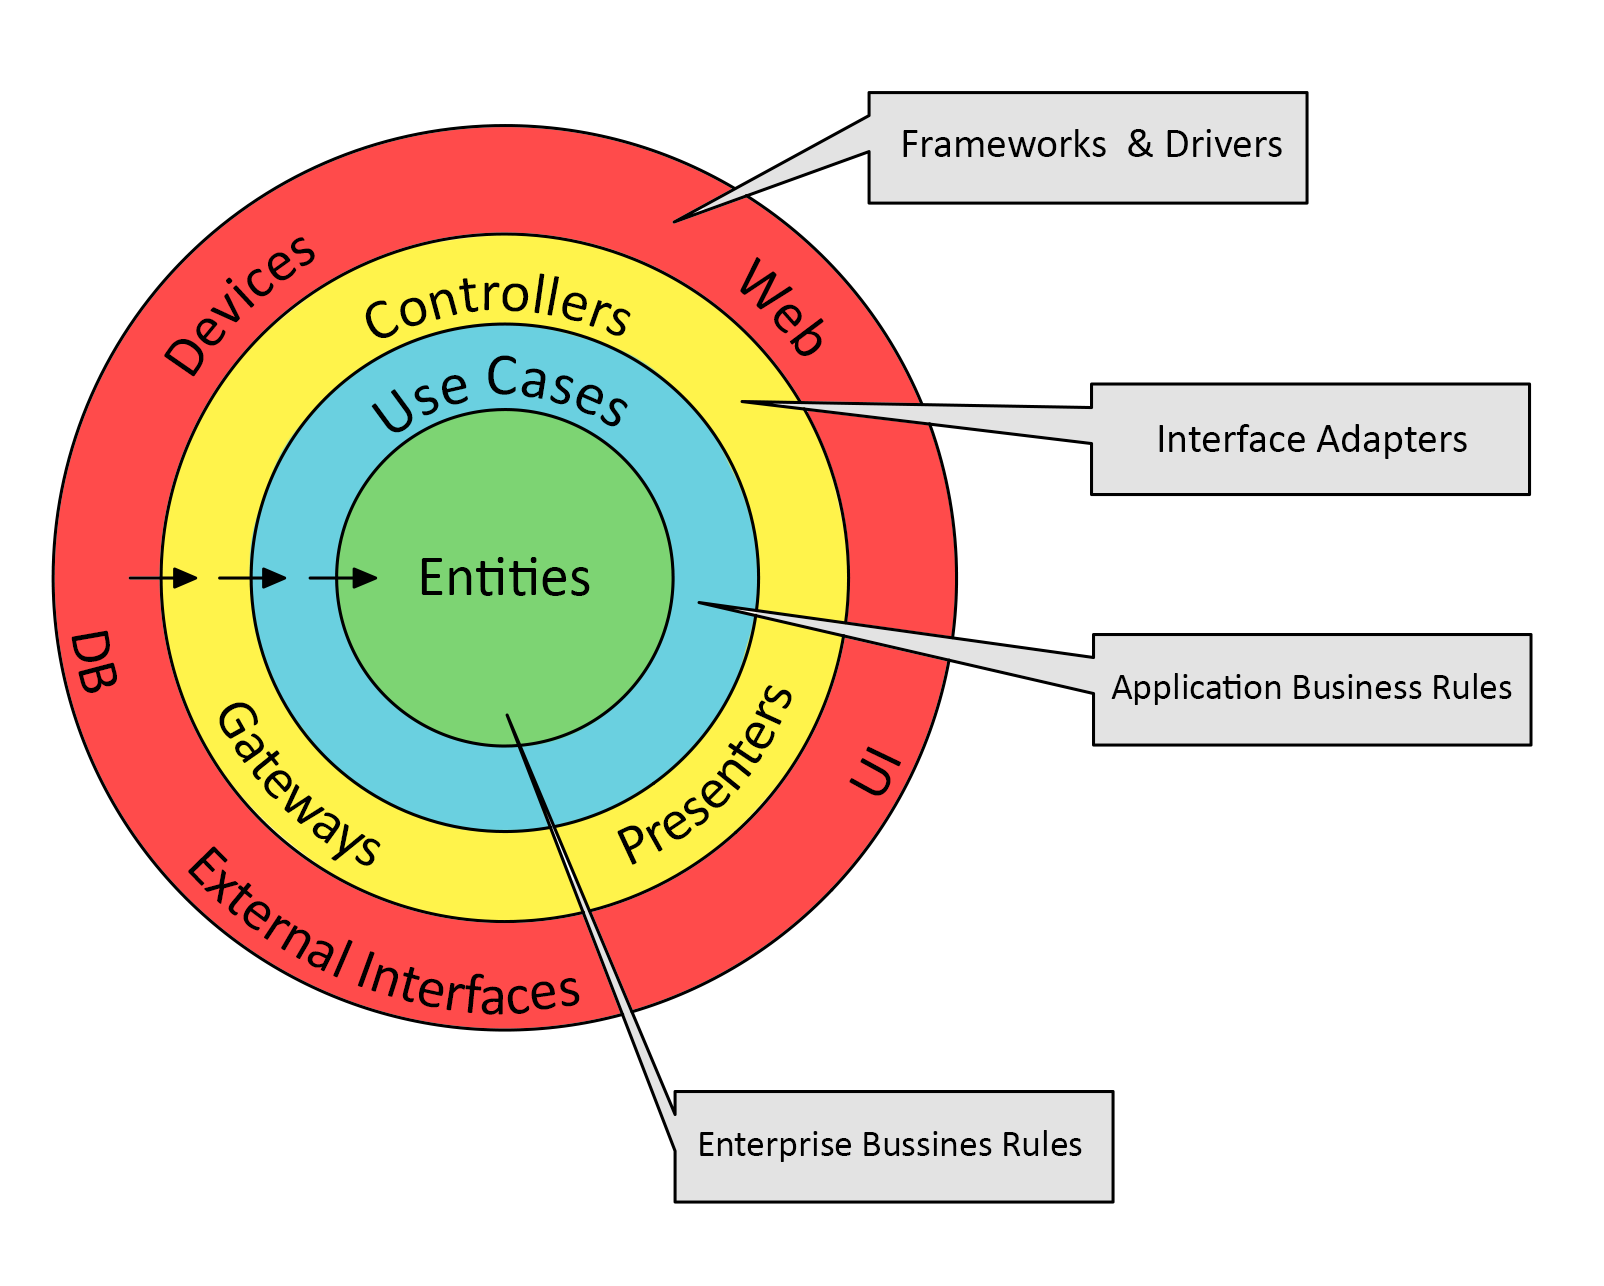
\includegraphics[width=0.45\textwidth]{clean.png}


\end{document}
